\chapter{Incorporating Recency in Web Search}
\label{ch:webranking}

Currently, the commercial search engine ranks documents according to their relevance to the query. As mentioned earlier, in this work we are upgrading an existing commercial search engine prototype to support recency as well. To further improve the quality of the search engine, we introduce the recency component on the query and the document side. The rest of this chapter first outlines the architecture of the commercial search engine, then describes in detail how the two machine-learning models explained in Chapters \ref{ch:doc} and \ref{ch:query} are integrated.

\section{Search Engine Architecture}

The architecture of a search engine begins with crawling documents from the Web and ends with retrieving and ranking a subset of documents that best match a given search query. This can be done in multiple stages, and we identify the main stages as crawling, document selection, indexing, and ranking. Furthermore, the stages can be divided into two different groups: offline and online. An offline stage is query-independent and can be done in an offline manner, i.e., once in the beginning and later only when needed. On the other hand, online stages are query-dependent and are run any time a query is submitted. A high-level overview of ranking stages of the commercial search engine is shown in Figure \ref{fig:arch}.

The indexing and ranking stages are supported by Elasticsearch.\footnote{\url{https://www.elastic.co/products/elasticsearch}.} Described in \citep{gormley2015elasticsearch}, Elasticsearch is a distributed, scalable, real-time search and analytics engine. It is built on top of Apache Lucene,\footnote{\url{https://lucene.apache.org/core/}.} a search-engine library written in Java. Elasticsearch uses Lucene internally for indexing and searching, but extends the usability by exposing an easy-to-use RESTful API. The indexing and ranking stages are explained in more detail in their respective sections.

\begin{figure}
  \centering
  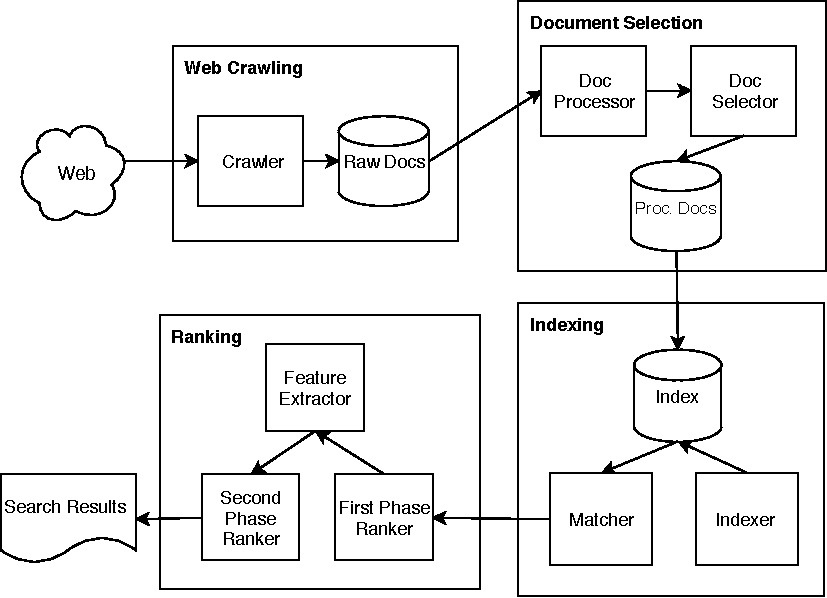
\includegraphics[width=\linewidth]{img/webranking.pdf}
  \caption{High-level architecture of the commercial search engine.}
  \label{fig:arch}
\end{figure}

\subsection{Web Crawling}
A crawler (or spider, robot, etc.) is a program that traverses the Web and downloads raw documents to a database. The two main tasks of a crawler are discovery and download of new pages and refreshing of the existing pages. The simplest approach is to start with a seed set of URLs, download the pages the URLs point to, then scan these pages for new links, add them to the queue of pages to be crawled, and repeat the process.

The crawler is an important component of a search engine, especially with regard to recency. For example, if there has been a breaking event and users search for it, if the crawler still has not crawled the relevant documents, they cannot be shown to the user. Therefore, a good crawler must download content fast enough so it does not become the bottleneck of the entire process.

\subsection{Document Selection}
The crawler can download a very large and diverse amount of content from the Web. However, not all of that content is useful. For example, we do not want to waste resources processing spam content. Therefore, the document selection stage filters out unnecessary documents, and stores the rest to be indexed. This stage consists of two modules: \texttt{Document Processor} and \texttt{Document Selector}. 

\texttt{Document Processor} is in charge of boilerplate removal and feature extraction. Boilerplate removal implies removing boilerplate parts from the Web page content (e.g., menus, footer, side bar) and unrelated parts (e.g., adverts, related articles). Consequently, we are left with a ``clean'' HTML, and we can extract features from the HTML and URL of the page, such as the number of tags and characters in the HTML, number of links, length of the link, etc.

\texttt{Document Selector} performs filtering of unwanted documents. It is a machine-learned regression model using Gradient Boosted Decision Trees (GBDT) to predict a document score. The features used are extracted from the HTML and the URL of the document. If the score of a document is below a certain threshold, it is discarded. Otherwise, the document is passed to the indexing stage. The scores are stored in a database, and the low-quality documents are removed periodically from the \texttt{Raw Docs} database.

\subsection{Indexing}
After a document is processed and stored in the \texttt{Processed Docs} database, it is sent to the indexing stage. Generally speaking, an index is a data structure that provides efficient retrieval for a given query. As mentioned earlier, this stage is handled by Elasticsearch and is run on an Elasticsearch cluster.

In Elasticsearch, documents are stored in an index as JSON objects which contain zero or more fields, or key-value pairs. In the \texttt{Document Selection} stage, \texttt{Document Processor} extracted features from the document content and its URL. These features are injected into the Elasticsearch index as key-value pairs in the document JSON.

An example of a simple keyword search query and a response from an index in Elasticsearch is shown in Listing \ref{es-search}. Additionally, Elasticsearch provides a Query DSL (Domain Specific Language) based on JSON to define queries, which is the way we query our indexes. An example of such query is shown in Listing \ref{es-search2}.

\begin{lstlisting}[language=json,firstnumber=1,caption=Example of a keyword search query and response in Elasticsearch., label=es-search]]
curl -XGET localhost:9200/books/_search?q=elasticsearch
{
  "took" : 2, "timed_out" : false,
  "_shards" : { "total" : 5, "successful" : 5, "failed" : 0 },
  "hits" : {
    "total" : 1, "max_score" : 0.076713204,
    "hits" : [ {
      "_index" : "books", "\_type" : "book", "\_id" : "1",
      "_score" : 0.076713204, "_source" : {
        "title" : "Elasticsearch - The definitive guide",
        "authors" : [ "Clinton Gormley", "Zachary Tong" ],
        "started" : "2013-02-04", "pages" : 230
      }
    } ]
  }
}
\end{lstlisting}

\begin{lstlisting}[language=json,firstnumber=1,caption=Example of a search query specified in DSL in Elasticsearch., label=es-search2]]
curl -XGET 'localhost:9200/books/book/\_search' -d '{
  "query": {
    "filtered" : {
      "query" : {
        "match": {
          "text" : {
            "query" : "To Be Or Not To Be",
            "cutoff_frequency" : 0.01
          }
        }
      },
      "filter" : {
        "range": {
          "price": {
            "gte": 20.0
            "lte": 50.0
   ...
  }
}'
\end{lstlisting}

The underlying data structure Elasticsearch uses for its index is the inverted index, designed to allow fast full-text searches. An inverted index consists of a list of all the unique words that appear in any document, and for each word, a list of the documents in which it appears. For example, if we have two documents $D_1$ = \textit{Madrid is the capital of Spain} and $D_2$ = \textit{Barcelona is the capital of Catalonia}. To create an inverted index, we first split the contents of each document into separate words, or tokens, normalize them, create a sorted list of all the unique tokens, and then list in which document each term appears. An example of such inverted index is shown in Table \ref{tb:inv-index}. If we want to search for \textit{capital spain}, we just need to find the documents in which each tokens appears, in this case the count is 2 for $D_1$, and 1 for $D_2$, so document $D_1$ seems more relevant for this query.

\begin{table}[]
\centering
\caption{A simple example of an inverted index.}
\label{tb:inv-index}
\begin{tabular}{@{}ccc@{}}
\toprule
Token & $D_1$ & $D_2$ \\ \midrule
barcelona & - & x \\
capital & x & x \\
catalonia & - & x \\
is & x & x \\
madrid & x & - \\
of & x & x \\
spain & x & - \\
the & x & x \\ \bottomrule
\end{tabular}
\end{table}

The indexing phase is finished when the document has been preprocessed, and the features have been extracted and stored as fields in the JSON object representing it.

\subsection{Ranking}
After the document has been indexed, once a user query is submitted, the \texttt{Matcher} matches the documents for the query. The matching is done by performing a logical conjunction (operator \texttt{AND}) between all of the terms from the query and the content of the document. Once we identify matching documents for a query, we can score them and rank them.

The ranking stage takes care of computing the relevance scores of the matching documents for the query and ranking them. Since there could be potentially millions of matching documents, computing all of the scores can be quite expensive. Therefore, we resort to a two-stage ranking architecture, where the first phase is essentially a cheap, but effective filter. The idea is to use query-independent features in the first phase ranking, because they can be precomputed in an offline manner and accessed by a simple lookup at query processing time. The first phase ranking function assigns scores to all of the matching documents $N$, and we only take the top $M$ ($M << N$) for the next stage. Since we now have a substantially smaller subset of the initial matching documents, we can extract more sophisticated and computationally expensive features. Finally, the second phase ranking function produces the ranking of the documents that are shown to the user.

We use and customize the Elasticsearch Learning to Rank plugin\footnote{\url{https://github.com/o19s/elasticsearch-learning-to-rank}.} for storing features, training datasets, models, and ranking the documents. We use the RankLib library\footnote{\url{https://sourceforge.net/p/lemur/wiki/RankLib/}.} to train the ranking models. Each model is described in its respective section as follows.

\subsubsection{First Phase Ranking}
In the first phase, we extract a combination of query-dependent and query-independent features. As described by \citet{cambazoglu2010early}, the first phase is used for selecting a small subset of potentially relevant documents from the entire collection. The typical features in this stage are:
\begin{itemize}
	\item \texttt{DocScore:} The score of the document produced in the Document Selection stage by the \texttt{Document Selector}. This score is also used as an indicator if we should index a document or discard it;
    \item \texttt{BM25(query, content):} The score of the $BM25$ function between the query and the content of the document.
\end{itemize}

The $\text{BM}25$ function \citep{robertson1996okapi} is a ranking function that can be computed automatically, without needing any relevance information. Given a query $Q$ containing keywords $q_1, ..., q_n$, the BM25 score of a document $D$ is:
\[ \text{BM}25(Q, D)=\sum _{i=1}^{n}{\text{IDF}}(q_{i})\cdot {\frac {f(q_{i},D)\cdot (k_{1}+1)}{f(q_{i},D)+k_{1}\cdot \left(1-b+b\cdot {\frac {|D|}{\text{avgdl}}}\right)}} \]

\noindent Here, $f(q_i, D)$ is $q_i$'s term frequency in the document $D$, $|D|$ is the length of the document $D$ in words, and $avgdl$ is the average document length in the text collection from which documents are drawn. Moreover, $k_1$ and $b$ are free parameters, and their default value in Elasticsearch is $k_1 = 1.2$ and $b = 0.75$. $\text{IDF}(q_i)$ is the inverse document frequency weight of the query term $q_i$. It is usually computed as:
\[ \text{IDF}(q_i) = \log \frac{N - n(q_i) + 0.5}{n(q_i) + 0.5} \]

\noindent Here, $N$ is the total number of documents in the collection, and $n(q_i)$ is the number of documents containing $q_i$.

Finally, we rank all the matching documents according to their first phase score, and get the top $M$ results, where $M << N$.

\subsubsection{Second Phase Ranking}
Contrary to the scoring function in the first phase, the second phase function is more complex. Since we only have a subset of documents to rank, we can afford extracting more computationally heavy features and training a more sophisticated model. The ranking produced by this model is the final ranking shown to the user. The model uses hundreds of features. Examples of different feature types are listed as follows:

\begin{itemize}
	\item \texttt{Query string.}\ Number of words, boolean features, etc.
    \item \texttt{URL string.}\ URL length, slash count, etc.
    \item \texttt{Document content.}\ Number of pictures, different tags, etc.
    \item \texttt{Content classification.}\ Output of classifiers of document content for spam, malware, adult content, etc.
    \item \texttt{Content-query relevance.} $\text{BM}25$ scores for query-title, query-URL, query-body, etc.
    \item \texttt{Content-query similarity.}\ Jaccard similarity or edit distance between the query and title, URL, etc.
    \item \texttt{Web graph.}\ PageRank, TrustRank, indegree, outdegree, etc.
    \item \texttt{Wikipedia.}\ Wikipedia page view count, references from Wikipedia, etc.
    \item \texttt{Traffic data.}\ The Alexa Traffic rank.\footnote{\url{https://www.alexa.com/siteinfo}.}
    \item \texttt{Document score.}\ Computed by the \texttt{Document Selector} model, trained using query-independent features.
    \item \texttt{First phase score.}\ Computed according to the ranking model in the first phase.
\end{itemize}

The offline features (query-independent) are computed and injected into the Elasticsearch index as document fields. The online features (query-dependent) are computed at query processing time using our customized Elasticsearch ranking plugin.

In this work, we introduce a type of features called \texttt{Recency features}, consisting of predicted document age and predicted query recency sensitivity. The document age feature is computed offline and injected into the ES index, whereas the query recency sensitivity feature should be computed at query processing time.

\section{Offline Experiments and Results}
In this section, we explain how we integrate the models explained in Chapters \ref{ch:doc} and \ref{ch:query} with the existing multi-stage ranking architecture. Our goal is to investigate whether the addition of recency features improves the overall ranking.

Both recency models, document age prediction and query recency sensitivity, are developed in a Hadoop cluster, and the extracted features and predictions are stored in HDFS. Apache Hadoop\footnote{\url{http://hadoop.apache.org/}.} is a free, open source, Java-based programming framework for distributed processing of large data sets across clusters of computers. Hadoop provides its own file system, called Hadoop Distributed File System (HDFS). Moreover, Hadoop handles job scheduling and cluster resource management, as well as parallel processing of large data sets. Both models run in Spark,\footnote{\url{http://spark.apache.org/}.} a fast and general compute engine for Hadoop data. The query recency sensitivity model is written in Python, using PySpark,\footnote{\url{https://spark.apache.org/docs/0.9.0/python-programming-guide.html}} the Spark Python API. The document age prediction model is written in Scala, which is supported natively in Spark.

\subsection{Model Integration}
Figure \ref{fig:docmodel} shows the integration of the document age prediction model into the existing ranking architecture. As described in Chapter \ref{ch:doc}, the ground truth is obtained by querying Memgator, an external web service. The script to build the ground truth, and the script to extract features are both written in Scala, run in Spark on the Hadoop cluster, and save the output data to HDFS. 

The document age model training module is written in Python to make use of XGBoost's Python API in scikit-learn.\footnote{\url{http://scikit-learn.org/stable/}.} We also run it on the Hadoop cluster, and save the predicted values to HDFS. Next, the Elasticsearch Feature Injector runs in Spark to read the predicted document last update time and inject it to Elasticsearch's index. Finally, we extend the Elasticsearch ranking plugin to calculate the document age as $currentTime - documentLastUpdateTime$ when queried (during the ranking models' training time).

\begin{figure}
  \centering
  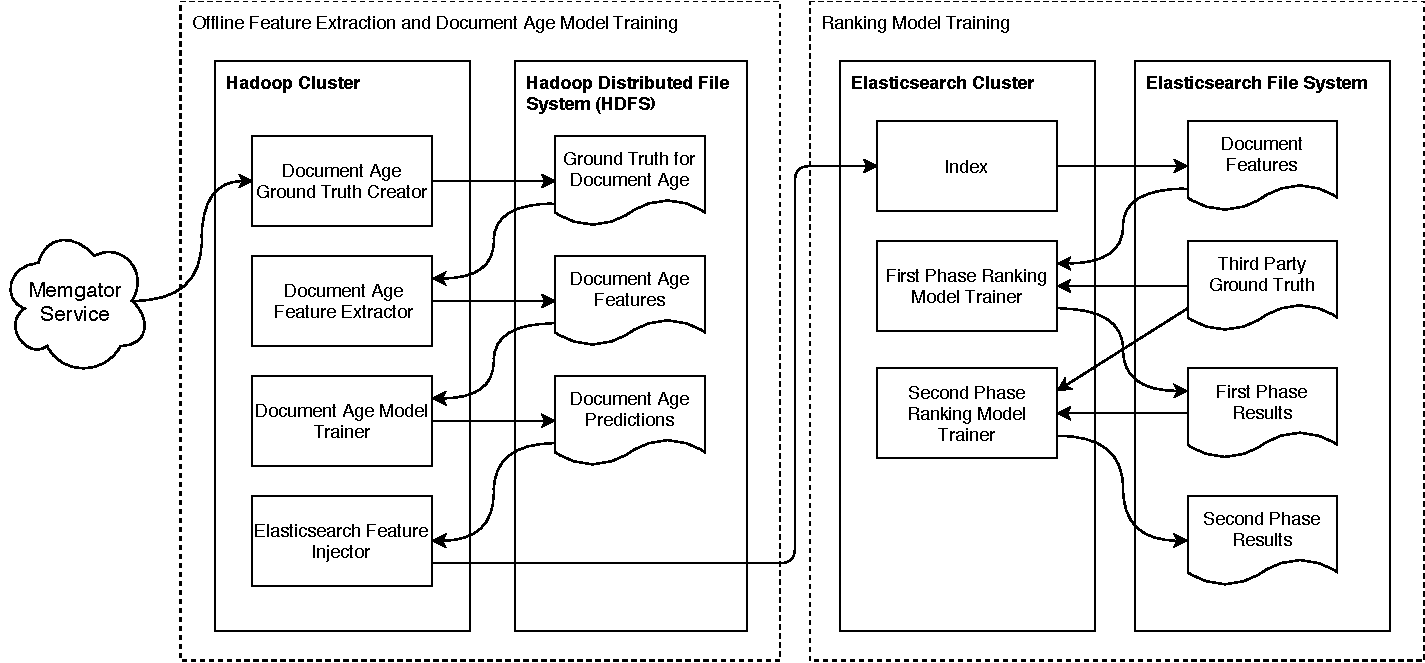
\includegraphics[width=\linewidth]{img/docmodel.pdf}
  \caption{Integration of the document age prediction model into the existing ranking pipeline.}
  \label{fig:docmodel}
\end{figure}

Figure \ref{fig:querymodel} shows the integration of the query recency sensitivity model into the existing ranking architecture. This model is described in detail in Chapter \ref{ch:query}. It is more complicated than the previous model in terms of external calls, because the corpora needed to build the language models is obtained from external sources such as Twitter and the query log. The ground truth is created by a PySpark script run in Spark on the Hadoop cluster that automatically labels queries according to the retrieved web snippets, and stores the output to HDFS.

The module that mines the Twitter corpus is a combination of Bash scripts (to retrieve the tweets using \texttt{twarc} and to extract the data) and PySpark (to filter and process the data, and save it to HDFS). The module that mines the query log corpus is a PySpark script that runs in Spark on the Hadoop cluster and saves the output to HDFS. The module that creates language models from both types of corpora is a Bash script which saves the resulting language models to HDFS. Next, the feature extractor is a combination of Bash scripts (to download the language models locally and to predict the language model feature type values) and PySpark (to extract the other feature type values).

Next, we need to inject the predictions of the query recency sensitivity model to the existing ranking pipeline. Since these predictions are related to the query itself, not the document, they cannot just be injected to the document index. Therefore, we inject them to our third party ground truth file used for training the ranking models. This is done by a Bash script that runs on the Elasticsearch cluster. The ground truth file consists of query-document pairs, so we simply append the query recency sensitivity score to each query-document pair. Finally, the recency sensitivity score is used as a feature in both the first- and second-phase ranking models.

\begin{figure}
  \centering
  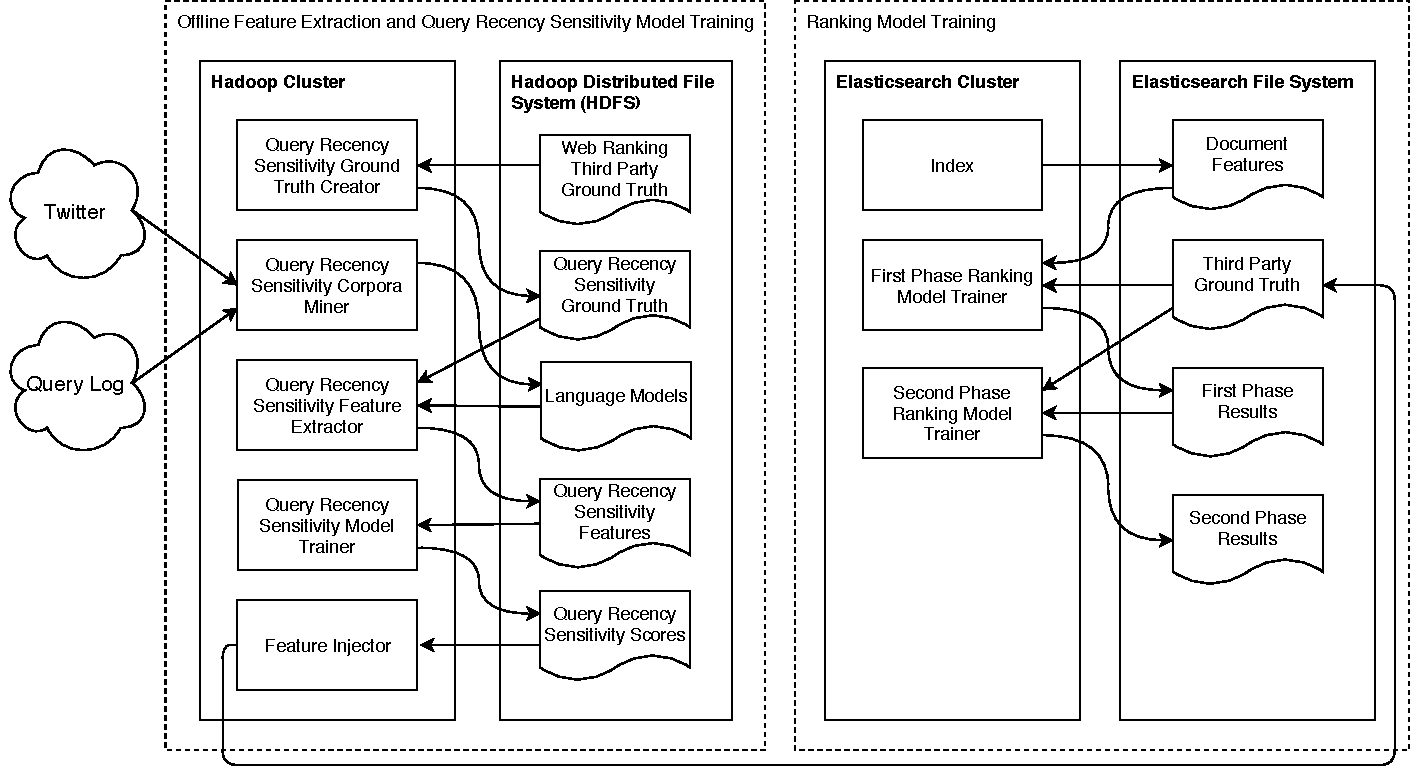
\includegraphics[width=\linewidth]{img/querymodel.pdf}
  \caption{Integration of the query recency sensitivity model into the existing ranking pipeline.}
  \label{fig:querymodel}
\end{figure}

\subsection{Recency Ranking Results}
The initial research question we asked ourselves is whether introducing recency features boosts the overall ranking performance. Since we are interested in the end result, or the quality of the search results shown to the user, we report the performance of the second-phase ranking model (which, in turn, also depends on the first-phase model, since its output is used as a feature).

Table \ref{tb:res} shows the evaluation of different ranking models. The evaluation metric used is NDCG@10 with respect to a third party search engine. The first model, denoted as F, is the model without any recency features. When adding just the document age feature (model F+1), we observe an increase in NDCG@10 of 0.35\%. This means that the model is now able to capture recency on the document side, but still not on the query side. In other words, it might learn to favour more recent documents in general, irrespective of the query. Furthermore, we add the query recency sensitivity score (model F+2), an observe an total increase in NDCG@10 of 0.48\%. Now, the model is able to learn to what extent to favour recent documents depending on the query. For example, if the query recency sensitivity score is low, there is no need to boost more recent documents. On the other hand, if the query recency sensitivity score is high, the ranking should be different than the one so far, without taking recency into account. In other words, more recent documents should be favoured.

Overall, we have introduced only two new features to the existing hundreds of features, and gained 0.48\% improvement in NDCG@10. Moreover, we evaluated the feature importances, shown in Table \ref{tb:f-imp-doc}. We can see that the model picks both features pretty early, as indicated by the rank of the tree they first appeared in. Therefore, the features are significant to the model's increase in performance.

\begin{table}[]
\centering
\caption{Evaluation of the recency feature importances in the second-phase ranking model.}
\label{tb:f-imp-doc}
\begin{tabular}{@{}ccccc@{}}
\toprule
Model & Feature name & Normalized feature rank & First appeared tree \\ \midrule
F+1 & documentAge & 0.72 & 541 (out of 2460) \\
F+2 & documentAge & 0.72 & 541 (out of 2937) \\
F+2 & queryRecencySensitivity & 0.73 & 660 (out of 2937) \\ \bottomrule
\end{tabular}
\end{table}

\begin{table}[]
\centering
\caption{Evaluation of the second-phase ranking model. Model F does not contain recency features, model F+1 contains the document age feature, and model F+2 contains both the document age feature and the query recency sensitivity score.}
\label{tb:res}
\begin{tabular}{@{}ccc@{}}
\toprule
Model & \multicolumn{1}{l}{Number of trees} & Improvement of NDCG@10 \\ \midrule
F & 1657 & - \\
F+1 & 2460 & 0.35\% \\
F+2 & 2937 & \textbf{0.48\%} \\ \bottomrule
\end{tabular}
\end{table}

\section{Online Integration and Future Work}
The previous section describes how we introduce the two recency features to the existing ranking models in an offline fashion. In other words, in that setup we are only training and evaluating the models. In an online, production setting, we want to be able to calculate these features on the fly. More specifically, when a user submits a query to the search engine, the document age model and the query recency sensitivity model must output a prediction.

Since the document age prediction model is not query-dependent, the online prediction involves calling the function in our Elasticsearch ranking plugin to calculate the document age with respect to the query submission time and the already injected document last update time, which is already supported.

However, for the online prediction of the query recency sensitivity model, we should already have the language models constructed and ready to use. This means we must already have the Twitter and query log corpora in place. As a reminder, we build language models based on the last day, week, and last two weeks (in case of tweets) or last month (in case of the query log). So, one challenge is to keep the language models fresh by updating the corpora they need daily. Another challenge, which has not been solved at to the time of writing, is to calculate query-dependent features in Elasticsearch which involve a call to an external store where the features would be located. This is a limitation of the ranking plugin we are using. Nevertheless, we are certain this feature will be supported soon, and the integration of it remains as future work. An example of an end-to-end online pipeline is shown in Figure \ref{fig:online}.

\begin{figure}
  \centering
  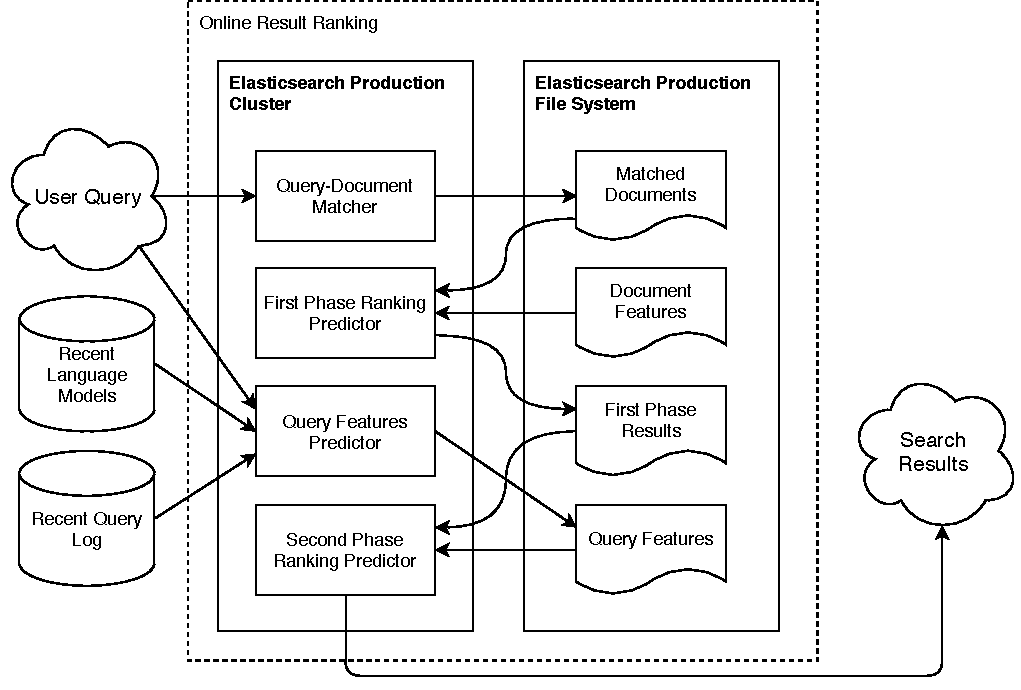
\includegraphics[width=\linewidth]{img/online.pdf}
  \caption{End-to-end pipeline for online result ranking.}
  \label{fig:online}
\end{figure}